% NESSF 2014 proposal

\documentclass[12pt]{article}

%% Use pdfTex to insure the margin sizes in Windows

\usepackage{natbib}
%\usepackage{natbib,natbibspacing}
\setlength{\bibsep}{1pt} % spacing for bibliography items
\citestyle{aa} % apj type
%\citestyle{plain} % number style
\usepackage{multicol} % multicolumns for references

% try smaller section title fonts
\usepackage{sectsty}
\sectionfont{\large}
\subsectionfont{\normalsize}

\pdfpagewidth=8.5in
\pdfpageheight=11in

\setlength\topmargin{-0in}
\setlength\headheight{0in}
\setlength\headsep{0in}
\setlength\textheight{9in}
\setlength\textwidth{6.5in}
\setlength\oddsidemargin{0in}
\setlength\evensidemargin{0in}

\usepackage{mathrsfs}
\usepackage{amsmath,amssymb}
\usepackage{verbatim}
\usepackage{wrapfig}

\usepackage{enumitem}

% journal names
\usepackage{aas_macros}

\newcommand{\beq}{\begin{equation}}
\newcommand{\eeq}{\end{equation}}
\def\etal{~et~al.~}
%\def\mps{m~s$^{-1}$}
\def\mps{m/s}
\def\msini{M\sin{i}}
\def\mjup{M_{\rm Jup}}
\def\msol{M_{\odot}}
\def\mearth{M_{\oplus}}
\def\degree{^{\circ}}
\def\leq{\leqslant}
\def\geq{\geqslant}
\def\kepler{{\it Kepler}}
\def\minerva{MINERVA}
\def\hrs{HET/HRS}
\def\keck{Keck/HIRES}

\usepackage{graphicx}
%\usepackage[pdftex,bookmarks, % add hyperlinks
%colorlinks,
%plainpages=false]{hyperref}

\begin{document}

%\tableofcontents
%\newpage

%%%%%%%%%%%%%%%%%%%%%%%%%%%%%%%%%%%%%%%%%%%%%%%%%%%%%%%%%%%%%%%%%%%%%%%%%%%%%%%%%%%%%%%%%
% title
\title{\vspace{-45pt} \bf \Large Finding the Lowest Mass Exoplanets with
  \\ Improved Radial Velocimetry \vspace{-6pt}}
\author{\normalsize Sharon Xuesong Wang}
\date{}
\maketitle

%%%%%%%%%%%%%%%%%%%%%%%%%%%%%%%%%%%%%%%%%%%%%%%%%%%%%%%%%%%%%%%%%%%%%%%%%%%%%%%%%%%%%%%%%
\vspace{-30pt}
\section{Overview}

% An overview of awesomeness of finding low-mass exoplanets.
The great synergy between NASA's \kepler\ mission and the ground-based
radial velocity (RV) surveys has made ground-breaking discoveries of
exoplanets, including many interesting low-mass \citep{marcy2014} and
likely rocky planets \citep{weiss2013} such as Kepler-78b, the first
exoplanet known to have radius and mass very close to Earth's
\citep{howard2013,pepe2013}. In the post-Kepler era, radial
velocimetry will continue to play a key role in validating Kepler
candidates and measuring their masses, as well as discovering
exoplanets independently.

% But... precise RV is yet to be more precise.
However, the current precision of radial velocimetry (0.5--1~\mps)
acts as one of the major limiting factors in detecting exoplanets with
even lower masses or rocky planets further out in the orbit,
especially in or near the Habitable Zone. Breaking this limit is
critical for enriching the diversity of the current exoplanet ensemble
towards the lower mass end, and it is a necessary step towards finding
Earth-mass exoplanets in the Habitable Zone around Sun-like stars,
which requires an RV precision of $\sim$0.1~\mps.
% ZZZ add number of kepler candidates with mass measurements with RV
% ZZZ add the current mass record holders 
% ZZZ doesn't feel like a very strong `but...'; add more on necessity
% of our work.

% What we propose to do
\textbf{We propose to improve the RV precision of several leading RV
  instruments through correction of systematic errors, with the aim to
  find the lowest mass exoplanets.} Improved radial velocimetry will
also enable better characterization of the current known low RV
amplitude planetary systems. Moreover, eliminating instrumental
systematic errors will help in isolating the RV signals induced by
stellar activities and promote a better understanding of the stellar
RV jitter, which is also crucial for finding lower mass exoplanets.


%%%%%%%%%%%%%%%%%%%%%%%%%%%%%%%%%%%%%%%%%%%%%%%%%%%%%%%%%%%%%%%%%%%%%%%%%%%%%%%%%%%%%%%%%
\vspace{-3pt}
\section{Expected Scientific Outcome and Impact}

% overall
Our work will directly improve the RV precision of the two leading RV
instruments on two 10-meter-class telescopes: Keck and the
Hobby-Eberly Telescope (HET). The large collecting areas of these
telescopes make them the ideal facilities for carrying out large and
deep surveys around bright or faint stars, as well as for extensive
follow-up observations on \kepler\ planet candidate systems. Our work
will also improve the RV precision of two instruments on
smaller telescopes: CHIRON and the upcoming MINiature Exoplanet RV
Array (\minerva). Designed for carrying out dedicated surveys with
extremely high RV precision, these two instruments will provide
valuable high cadence data on nearby and bright stars, which are the
best targets for planetary atmosphere characterization studies.

% Keck
\textbf{Science with \keck: } The primary instrument we work with is
the High Resolution Echelle Spectrometer (HIRES) on Keck I (current RV
precision $\sim$1~\mps). Among the 432 RV discovered exoplanets,
\keck\ has contributed the most ($\sim$200). It has also contributed
to a great number of mass measurements of confirmed \kepler\ planets
--- in particular, \textit{most} of the low mass ones
\citep[e.g.,][]{gautier2012,gilliland2013,howard2013,marcy2014}. However,
its current RV precision is limiting its ability to detect lower mass
planets or planets with the same mass but further out in orbit
\citep[e.g.,][]{marcy2014}.

% Lots of low mass Kepler planets
Our work will improve the RV precision of \keck, and thus extend the
lower mass limit of the current exoplanet sample. This is especially
promising when considering the large candidate pool that
\kepler\ provides: among the $\sim$1600 KOIs with transit signals
suggesting a planet radius smaller than 2 Earth radii, there are
$\sim$260 whose host stars have \kepler\ magnitude $< 13$ and are thus
bright enough for Keck to follow up (compared with fewer than 10 such
targets with \kepler\ mag $< 9$ and thus accessible to HARPS-N; data
from exoplanets.org).

% Multi-planet systems to improve with Keck
Meanwhile, better RV precision will improve the characterization of
multiple-planet systems, especially the ones that host challenging low
RV amplitude planets/candidates and with potentially very active
dynamic interactions. We will reanalyze the RV data and perform
dynamic analysis on such systems, including the GJ 876 system, which
is the closest multi-planet systems to the Sun
\citep{marcy2001,rivera2005,rivera2010}, the $\upsilon$ Andromedae
system, the first multi-planet system discovered around main-sequence
star \citep{butler1999,wright2009,curiel2011}, as well as the GJ 581
system, which hosts the first claimed terrestrial-mass exoplanet in
the Habitable Zone (\citealt{vogt2010}, though these are under debate,
e.g.~\citealt{gregory2011,vogt2012,robertson2013}).

% HET
\textbf{Science with \hrs: } We will also improve another leading RV
instrument on a 10-meter-class telescope: the High Resolution
Spectrograph (HRS) on HET (current RV precision $\sim$3--5~\mps). With
multiple ongoing upgrades on \hrs\ (expected to finish in summer
2014), its throughput will be improved by a factor of $\sim$5, also
with the promise of higher RV precision of the new HRS. HET will
become the second telescope, besides Keck, capable of RV follow-up on
planet candidates discovered by \kepler. This will also benefit other
planet search programs on \hrs\ such as surveys on long-period planets
and multiple-planet systems.

% Minerva and CHIRON
\textbf{MINERVA and CHIRON: } Our work also has great synergy with two
very high RV precision instruments on smaller telescopes: the upcoming
\minerva\ and CHIRON on the 1.5m SMARTS telescope at CTIO. 

\minerva\ will consist of an array of four 0.7m telescopes and a
vacuum-sealed highly-stable spectrograph that will perform dedicated
RV monitoring on a carefully-selected ensemble of nearby stars. It is
expected to discover $\gtrsim 10$ Earth- to super-Earth-size planets
with orbital period of 1--100 days around nearby stars, with 3--5
expected to be in the Habitable Zones of their host stars
\citep{bottom2013,hogstrom2013}. Our work will prepare \minerva\ to
meet its targeted long-term RV precision of $\sim 0.8$~\mps.

CHIRON has demonstrated short-term RV stability of $\sim0.5$~\mps\ on
$\tau$ Ceti \citep{chiron2013}. The improvement we propose will help
CHIRON achieve long-term RV stability below 1~\mps\ and help validate
or characterize the potential planetary systems around $\tau$ Ceti
\citep{tuomi2013} and $\alpha$ Centauri B
\citep{dumusque2012,hatzes2013}, whoese planets (candidates) have RV
amplitudes on the order of $\sim 1$~\mps\ or even smaller.


%---------------------------------------------------------------------------------------
% RECYCLE BIN
\begin{comment}
% overview
The excellent synergy between NASA's \kepler\ mission and the
ground-based radial velocity (RV) surveys has made numerous
ground-breaking discoveries of exoplanets, including many interesting
low-mass and rocky planets
\citep[e.g.,][]{howard2013,pepe2013,marcy2014}. This has brought the
field of exoplanets into an exciting era with an inceasing sample of
small and potentially rocky planets \citep{weiss2013} with the great
promise towards the discovery of Earth analogs in the near future.

In the post-\kepler\ era, radial velocimetry will undoubtedly continue
to play a key role in validating \kepler\ candidates and measuring
their masses, as well as discovering exoplanets
independently. However, the current precision of radial velocimetry
(0.5--1~\mps) acts as one of the major limiting factors in detecting
exoplanets with even lower masses or rocky planets further out in the
orbit, especially in or near the Habitable Zone. Breaking this limit
is critical for pushing the lower mass boundary of the exoplanet
ensemble. It is also an absolutely necessary step towards finding
Earth-mass ($\mearth$) exoplanets in the Habitable Zone around
Sun-like stars, which requires an RV precision of $\sim$0.1 \mps.
  
The field of exoplanet is progressing in a fast pace towards the
discovery of Earth-like planets around other stars. During the past
decades, we have moved on from the age of booming discoveries of
Jupiter-mass exoplanets via radial velocimetry (add ref) to the
\kepler\ era where there are thousands of Earth- and super-Earth-size
exoplanet candidates (add ref). Moreover, great promises lie ahead with
future ground-based instruments (e.g., ESPRESSO; add ref) or space
missions (e.g., TESS; add ref).

\begin{itemize}[leftmargin=2.2em]
    \vspace{-3pt}
\item Improve the RV precision of Keck through eliminating known
  systematics and improved statistics.
    \vspace{-3pt}
\end{itemize}

% methodology overview
We propose to work on: removal of RV systematic errors / annual jitter
cause by the Earth's atmospheric absorption (telluric lines;
Section~\ref{sec:tell}); improvements in wavelength-dependent
statistical weighting in spectrum for RV extraction
(Section~\ref{sec:vanking}); validation of the RV calibrator, the
iodine atlas, using high-resolution echelle spectrograph
(Section~\ref{sec:fts}); and improvements in data reduction and
instrumental effect modeling for fiber-fed RV instruments
(Section~\ref{sec:ip}). 

% FTS
We took a 30\AA\ chunk of echelle absorption spectrum of
the iodine cell at the McDonald 2.1m telescope and compared it with
its FTS iodine atlas (also taken at KPNO in 1993 and thus can
represent the quality of the KPNO FTS spectra).

One key element in precise RV work with iodine is the ``ground truth"
of the absorption spectrum of the iodine cell, which is normally a
wavelength-calibrated, very high-resolution iodine atlas taken by a
Fourier Transform Spectrometer (FTS). Treated as the ``true and perfect
iodine spectrum", the FTS iodine atlas is used for modeling the iodine
lines in the observed stellar$+$iodine spectrum to anchor the absolute
wavelength solution and the spectrograph response function. Therefore,
an accurate and precise iodine atlas is crucial for achieving high RV
precision.

When extracting RVs from the stellar spectrum obtained through an
iodine cell, one relies on the modeling of the iodine lines using the
``true lines" in the iodine atlas to anchor the absolute wavelength
solution and the spectrograph response function (the ``spectral PSF").

Modeling the observed iodine lines using this ``ground truth" iodine
atlas anchors the absolute wavelength solution and the spectrograph
response function (the `spectral PSF' or instrumental profile, `IP')
when extracting RVs from the stellar spectrum.

Modeling the observed Iodine lines with the FTS scan spectrum anchors
the absolute wavelength solution and spectrograph response function
when extracting RVs from the stellar spectrum.

% an old section
\section{Relation to PI's Other NASA Grants}
The PI of this proposal, Dr.~Jason Wright, has received NASA Keck
time to search for long-period planet and multiple planet systems.
The PI has also received NASA Keck time to follow up a
\kepler\ planetary system with a strong TTV signal (Co-I Eric
Ford). Both of these programs will of no doubt benefit from the
improved Keck RV precision, and the upgraded \hrs\ is expected to
follow up some if not all of the long-period planet systems and
\kepler\ TTV systems in the future.

% itemized relevance to NASA
\begin{itemize}[leftmargin=1.5em]
  \vspace{-8pt}
\item ``to search for planets and planetary systems about
  nearby stars in our Galaxy": This is the direct science goal of our
  work. 
  \vspace{-5pt}
\item ``to determine the properties of those stars that harbor
  planetary systems": We will acquire high resolution spectra on
  planet host stars with \keck\ and \hrs\ for, e.g. the
  \kepler\ stars, as required by the RV technique. Improved RV
  precision will also help better understanding stellar activities and
  stellar RV jitter.
  \vspace{-5pt}
\item ``to determine the percentage of planets that are in or near the
  Habitable Zone of a wide variety of stars and to measure their
  orbits": Improved RV precision of \keck\ and \hrs\ will enable more
  detections of potentially rocky exoplanets in the Habitable Zone of
  their host stars, which is also the immediate goal of project \minerva.
  \vspace{-8pt}
\end{itemize}

\end{comment}
%---------------------------------------------------------------------------------------



%%%%%%%%%%%%%%%%%%%%%%%%%%%%%%%%%%%%%%%%%%%%%%%%%%%%%%%%%%%%%%%%%%%%%%%%%%%%%%%%%%%%%%%%%
\vspace{-3pt}
\section{Methodology}

% overall
Our approach for improving the RV precision is to eliminate the RV
systematic errors, one of the two major contributors to the 'RV
jitter' (the other being stellar jitter). Our pilot study has
identified several contributing factors to RV systematic errors, some
of which are being recognized and studied in detail \textit{for the
  very first time}. Some of these factors contribute to the RV error
budget at $\sim 1$~\mps\ level, and thus they set the floor of
long-term RV precision at 1~\mps\ if not carefully studied and
corrected for.

%---------------------------------------------------------------------------------------
\vspace{-3pt}
\subsection{Removing the Systematics Caused by Telluric
  Lines}\label{sec:tell}

% telluric lines act like stellar line impostors but don't shift
In precise iodine radial velocimetry, RVs are measured from the
differential shift of stellar lines between two stellar spectra.
Since all current RV instruments are ground-based, the stellar spectra
inevitably contain telluric absorption lines as from the light's
travel through Earth's atmosphere. These telluric lines impersonate
stellar lines but do not exhibit Doppler shifts caused by the Earth's
barycentric motion ($\sim$a few to tens of k\mps) and the planets. The
resulting ``peak-pulling" effect in the iodine analysis (see,
e.g.~\citealt{wright2013}) then manifests as an annual systematic
signal.

% before we thought it was ok, then we recognized and showed for the
% first time that it's not
For years, such problems caused by telluric lines were thought to have
been suppressed to a negligible level, because there are only few
telluric bands mostly with shallow lines within the working wavelength
region of iodine radial velocimetry (5000\AA--6000\AA). However, as
the RV precision improved over time and has approached
$\sim1$~\mps\ and better, the adverse effects of telluric lines have
emerged and become one of the current bottlenecks of precise radial
velocimetry. \textbf{This is demonstrated \textit{for the first time}
  through our preliminary study, and with some initial effort in
  telluric line masking, we were able to eliminate a visible amount of
  the systematic RV errors}, which is illustrated in Figure~\ref{fig:tell}.

\begin{figure}[thb]
  \vspace{-5pt}
  \begin{center}
    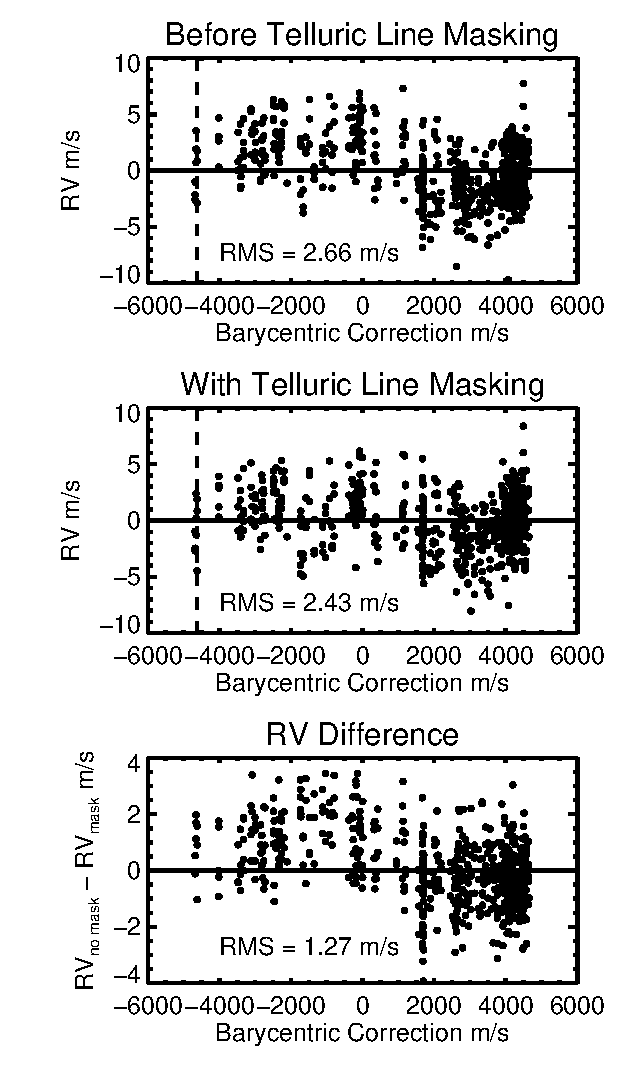
\includegraphics[scale=0.6]{telluric}
  \end{center}
  \vspace{-25pt}  
  \caption{Measured precise radial velocities of a standard star
    observed with \keck\ as a function of barycentric correction
    (i.e.~Earth's radial velocity away from the target). Our
    preliminary treatment of telluric lines has removed over
    1~\mps\ systematic noise.}
  \vspace{-8pt}  
  \label{fig:tell}
\end{figure}

Figure~\ref{fig:tell} shows that the long-term ($> 5$ years) RV RMS of
an RV standard star observed by \keck, HD 185144 ($\sigma$ Draconis),
is reduced from 2.66~\mps\ to 2.43~\mps\ --- an RMS of 1.08~\mps\ is
removed from the RV jitter ($\sqrt{2.66^2-2.43^2}$). The bottom panel
of Figure~\ref{fig:tell} illustrates the removed systematic errors,
which has a clear annual signal. The rest of the RV jitter may be due
to residual telluric line effects, intrinsic stellar jitter, other
unknown systematic errors, or even low RV amplitude planets.

% this is only the beginning - lots of improvements can be done!
We will further reduce the systematics caused by telluric lines in
several ways. For example, currently we are masking out the telluric
lines by using a naive simulated telluric spectrum based on the
elevation of Mauna Kea with nominal atmospheric compositions and
conditions. In the future we will employ empirical masks derived from
B star observations. Another example is that the RV extraction code is
not yet optimized to consistently produce a good fit in regions where
some of the pixels are being masked out due to telluric lines,
especially for the cases with large barycentric velocity shifts. A
more carefully-tuned $\chi^2$ minimization algorithm will allow us to
recover reliable RVs from \textit{all} segments of the iodine-laced
stellar spectrum, including those with significant telluric
contamination.

% also HET, MINERVA and CHIRON!
This work will naturally improve the RV precision of \hrs\ and
\minerva, as they share essentially the same RV extraction code
inherited from the \keck\ pipeline. Moreover, the sites of \hrs\ and
\minerva\ are at much lower elevations than Mauna Kea, which means
that the telluric line contamination probably causes more severe
systematic errors. We will also work with the CHIRON team to implement
the treatment for telluric lines to help CHIRON achieve higher
long-term RV precision.


%---------------------------------------------------------------------------------------
\vspace{-3pt}
\subsection{Improving Wavelength-Dependent Statistical Weights}\label{sec:vank}


\begin{wrapfigure}{r}{0.5\textwidth}
  \vspace{-35pt}
  \begin{center}
    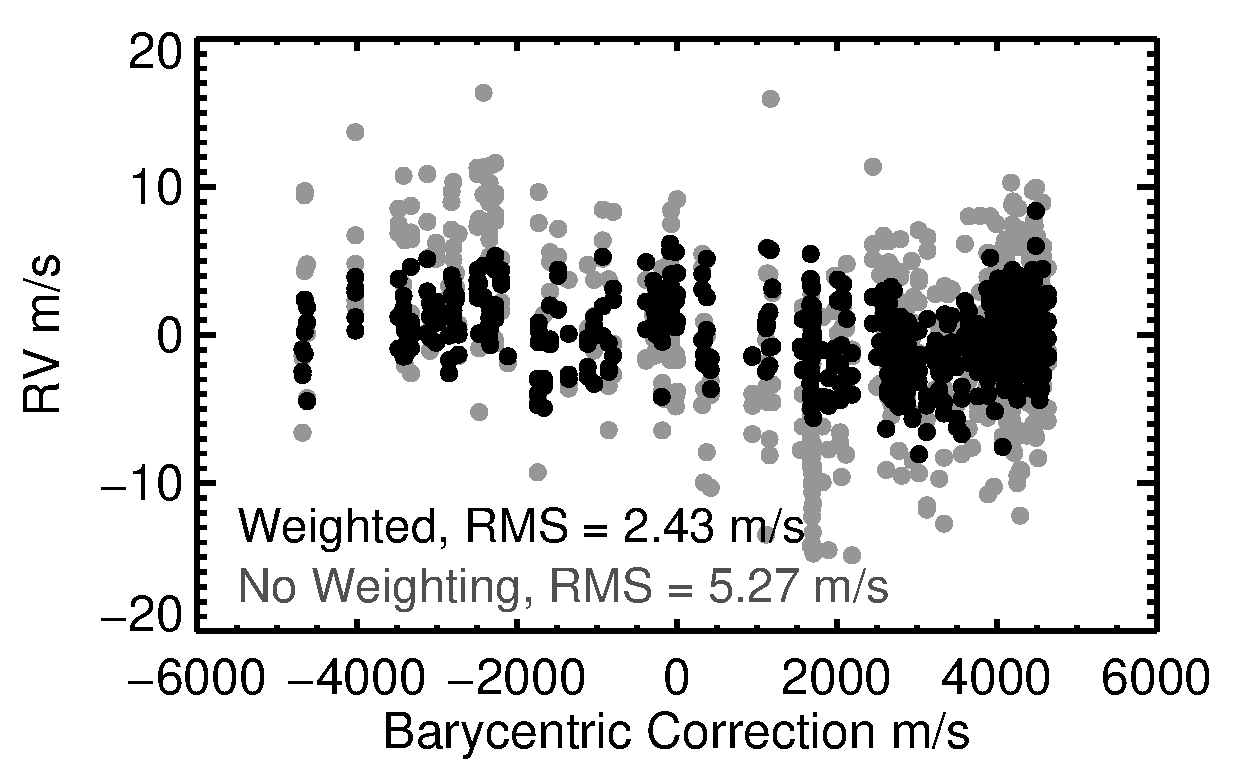
\includegraphics[width=0.47\textwidth]{vank}
  \end{center}
  \vspace{-25pt}  
  \caption{RV RMS of HD 185144 before (gray) and after (black) weighting.} 
  \vspace{-8pt}  
  \label{fig:vank}
\end{wrapfigure}

% what is weighting and its importance
The application of wavelength-dependent statistical weights is the
``secret sauce" of precise iodine radial velocimetry. It evaluates the
RV performance of each wavelength region across observations and
assigns them statistical weights before computing the final mean
RV. It also adjusts for the wavelength-dependent systematic offsets
and rejects outlier regions with poor RV RMS
performance. Figure~\ref{fig:vank} illustrates the crucial role of
this weighting scheme in precise RV.

% what we have learned and plan to do




%---------------------------------------------------------------------------------------
\vspace{-3pt}
\subsection{Validating the Calibrator: the Iodine Atlas}\label{sec:fts}

A ``ground truth" iodine atlas is crucial for the precise iodine radial
velocimetry. It is used for modeling the observed iodine lines in the
stellar$+$iodine RV observation to anchor the absolute wavelengths and
the spectrograph response function. Such a ``ground truth" atlas is
normally obtained through a Fourier Transform Spectrometer
(FTS). However, our recent work has revealed potential problems with
the quality of FTS iodine atlases.

We took a new FTS atlas of the \hrs\ iodine cell at NIST and compared
it with the old one (taken at KPNO in 1993), which showed that they
differ significantly in terms of wavelength solution, wavelength
dispersion scale, iodine line depths, and line depth ratios. Doppler
reductions on the RV standard star HD 185144 yield a RV jitter of
$\sim5$~\mps\ when using the new FTS atlas and $\sim4$~\mps\ with the
old one. This calls into questions of how ``true" any existing FTS
iodine atlas really is, and demands for an independent method to
validate them. \textbf{We propose to validate the quality of the FTS
  iodine atlases for the new \hrs\ and \minerva, and also for CHIRON
  and other RV instruments if necessary.}

We have found a method to independently validate the quality of FTS
iodine atlas, which is to take a high-resolution iodine absorption
spectrum in the ``real wavelength space" (as opposed to in Fourier
space with FTS) using an echelle spectrograph. We used the TS12 arm of
the Tull Spectrograph at the McDonald Observatory 2.7m telescope,
which has the matching spectral resolution to an FTS ($R \sim
500,000$). For our pilot study, we used the iodine cell at the
McDonald 2.1m telescope, whoese FTS atlas was also taken at KPNO in
1993 and thus can represent the quality of the KPNO FTS atlases.

\begin{wrapfigure}{r}{0.5\textwidth}
  \vspace{-35pt}
  \begin{center}
    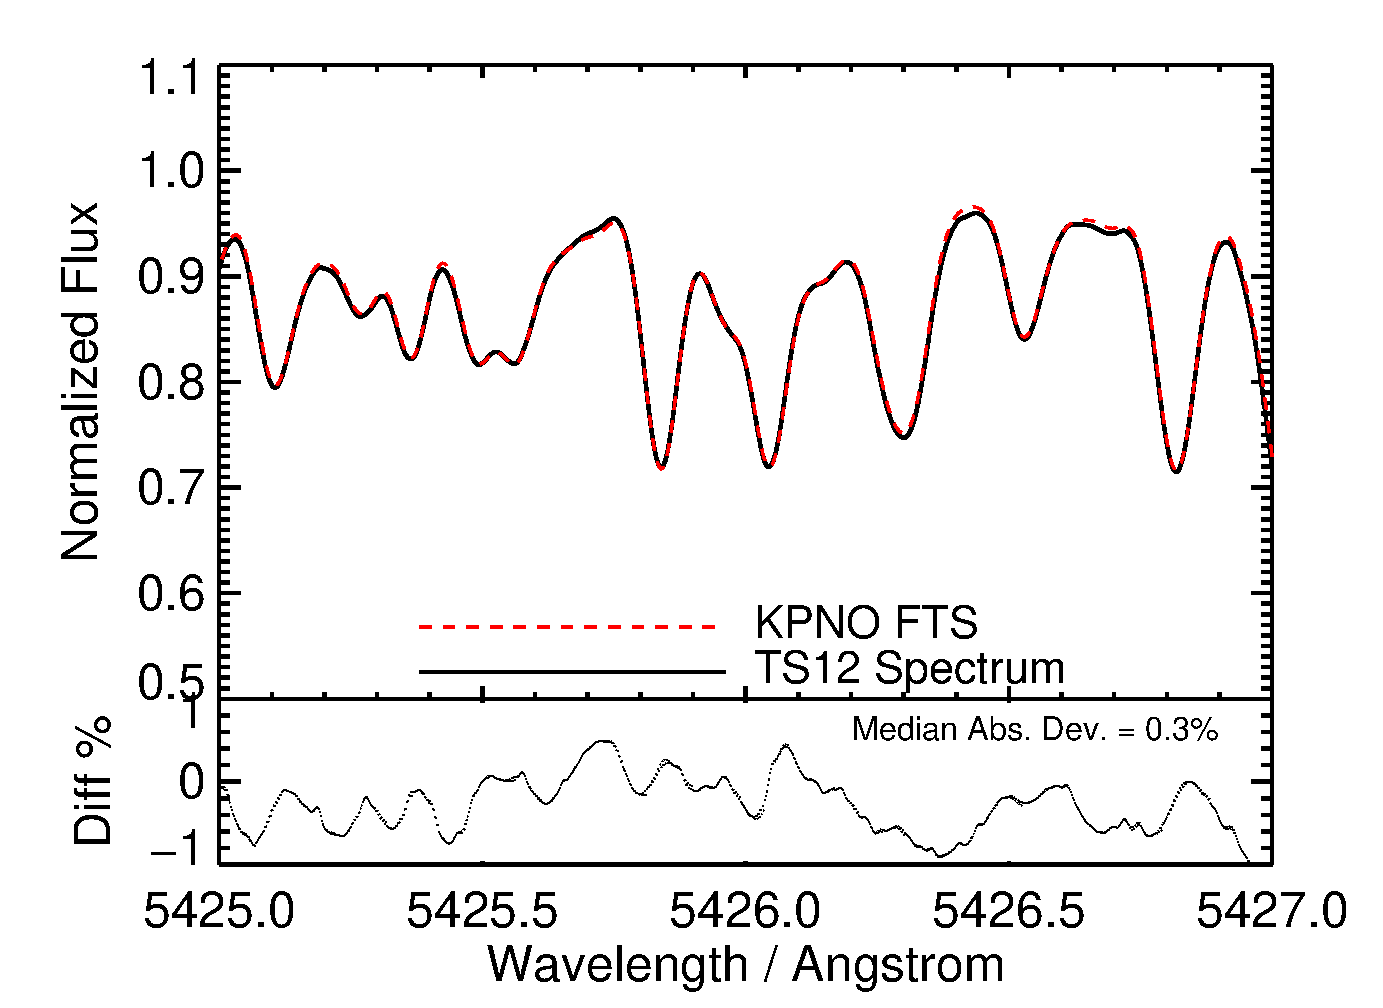
\includegraphics[width=0.47\textwidth]{fts}
  \end{center}
  \vspace{-25pt}  
  \caption{FTS iodine atlas compared with echelle spectrum, both
    at $R=60,000$.}  
  \vspace{-8pt}  
  \label{fig:fts}
\end{wrapfigure}

Figure~\ref{fig:fts} illustrates the comparison between the FTS iodine
atlas and the echelle spectrum (zoomed into a 2\AA\ chunk). It shows
that, when convolved down to resolution $R=60,000$ (typical resolution
of an star$+$iodine RV observation), the difference between the KPNO
scan and the echelle spectrum is very small considering photon-limited
errors and potential errors in flat fielding and scattered light
removal.

This demonstrates that we have found an independent and reliable
method to validate any FTS iodine atlas. Current and upcoming RV
instruments such as the new \hrs, \minerva, and CHIRON will need
validation for their FTS iodine atlases to eliminate one risk factor
that could potentially compromise the RV precision, which is our
proposed work here.

% not a very strong section...
%---------------------------------------------------------------------------------------
\begin{comment}
\vspace{-3pt}
\subsection{Improving Data Reduction and Instrument Modeling}\label{sec:ip}

This part is for improving RV of fiber-fed spectrographs: \hrs,
\minerva, and CHIRON.

The new \hrs\ is going to have a different spectral format, which is
very similar to what \minerva\ will have. We need to modify the data
reduction and doppler code for \hrs\ to adapt to it to ensure it
reaches the optimized precision. This will naturally also be
preparation work for \minerva. Addressing the challenge of flat
fielding for such spectral format will also help improve CHIRON.

Another crucial work is to model the instrumental profile of fiber-fed
spectrograph really well and to understand the problems that are
unique for fibers. IP is very important and \hrs\ is not doing very
well. We have acquired lots of engineering data on
\hrs\ to specially designed for modeling IPs and understanding modal
noise of fibers. Combined with years of engineering data and
experience with CHIRON, improvement on IP modeling is ahead. This is
also a natural preparation work for \minerva.

\end{comment}


 
%%%%%%%%%%%%%%%%%%%%%%%%%%%%%%%%%%%%%%%%%%%%%%%%%%%%%%%%%%%%%%%%%%%%%%%%%%%%%%%%%%%%%%%%%
\vspace{-3pt}
\section{Relevance to NASA's Objectives and Missions}

Broadly, our investigation addresses one of the science
objectives of NASA SMD, ``Discover the origin, structure, evolution
and destiny of the universe and search for Earth-like planets".

More specifically, this proposal is directly and closely relevant to
the Astrophysics Research Program, theme (iii) Exoplanet Exploration,
in the solicitation: \textbf{(1)``to search for planets and planetary
  systems about nearby stars in our Galaxy":} This is the direct
science goal of our work. \textbf{(2) ``to determine the properties of
  those stars that harbor planetary systems":} We will acquire high
resolution spectra on planet host stars with \keck\ and \hrs\ for,
e.g. the \kepler\ stars, as required by the RV technique. Improved RV
precision will also help better understanding stellar activities and
stellar RV jitter. \textbf{(3)``to determine the percentage of planets
  that are in or near the Habitable Zone of a wide variety of stars
  and to measure their orbits":} Improved RV precision of \keck\ and
\hrs\ will enable more detections of potentially rocky exoplanets in
the Habitable Zone of their host stars, which is also the immediate
goal of project \minerva.

Our work will also support current and future NASA missions and
enhance their scientific outcome: (1) {\bf the \textit{Kepler}
  mission}: Our work directly supports the \kepler\ mission through
candidate validation/confirmation, planetary mass measurements, TTV
target follow-up, and outer planet discovery using \keck\ and
\hrs. {\bf (2) TESS:} \keck, \hrs, and \minerva\ can all contribute
significantly to the follow-up programs of TESS. {\bf (3) JWST:}
Finding more lower mass exoplanets means more super Earths and Earth
analogs, which are the primary targets for JWST for planetary
atmosphere characterization.



%%%%%%%%%%%%%%%%%%%%%%%%%%%%%%%%%%%%%%%%%%%%%%%%%%%%%%%%%%%%%%%%%%%%%%%%%%%%%%%%%%%%%%%%%
%\newpage
%\addcontentsline{toc}{section}{References}
\vspace{-3pt}
\bibliographystyle{apj}	% (uses file "xxx.bst")
%\begin{multicols}{2}
{\small % smaller fonts for references
%{\footnotesize
\bibliography{references} }
%\end{multicols}

\end{document}
